
%%%%%%%%%%%%%%%%%%%%%%%%%%%
% IEEE Submission Dashboard - https://ieee.atyponrex.com/submission/dashboard
%%%%%%%%%%%%%%%%%%%%%%%%%%%

% \documentclass[10pt,journal,compsoc]{IEEEtran}
% \documentclass[lettersize,journal]{IEEEtran}
% \documentclass[letterpaper,journal]{IEEEtran}
\documentclass[journal]{IEEEtran}
% ==== Core packages (normalized) ====

% How to hide statements: 
%   - To enable  tags: \iftrue  and \fi
%   - To disable tags: \iffalse and \fi
% How to turn-on (or turn-off) page number:
%   - To turn-on  the page number: {plain}
%   - To turn-off the page number: {empty}
% Usage (Syntax): 
%   \documentstyle[twocolumn]{article}
%   \pagestyle{empty}
%    ...
%   \maketitle
%   \thispagestyle{empty}

% How to print the page number at each page 
\pagestyle{empty}

\usepackage[T1]{fontenc}
\usepackage[utf8]{inputenc}
\usepackage{microtype}
\usepackage{amsmath,amssymb}
\usepackage{amsthm}  % required for theorem environments
%\usepackage{amsmath}
%\usepackage{amssymb}
\usepackage{makecell}
%\usepackage{amsmath,amsfonts,amssymb,mathtools}
%\usepackage{amsthm}
\usepackage{graphicx}
\usepackage{booktabs}
\usepackage{siunitx}
\usepackage{xspace}
\usepackage{pifont}
% Checkmark / Xmark symbols
\newcommand{\cmark}{\ding{51}}
\newcommand{\xmark}{\ding{55}}

\usepackage{listings}
\usepackage{xcolor}
\usepackage{xurl}
\usepackage{url}


% Hyperlinks to content
% \usepackage[linktocpage=true]{hyperref}
% \usepackage{hyperref}
% \usepackage[nameinlink]{cleveref}
% \usepackage[hidelinks]{hyperref}
% TMC requirement (decision letter): "Text in any color other than black is not
% acceptable." Links remain active but are rendered black instead of blue.
\usepackage[colorlinks=true,linkcolor=black,citecolor=black,urlcolor=black]{hyperref}

\usepackage{cleveref}
%\usepackage{amsmath,amsfonts}
\usepackage{algorithmic}
\usepackage{algorithm}
\usepackage{array}
\usepackage[caption=false,font=normalsize,labelfont=sf,textfont=sf]{subfig}
\usepackage{textcomp}
\usepackage{stfloats}
\usepackage{verbatim}
\usepackage{cite}
%\hyphenation{op-tical net-works semi-conduc-tor IEEE-Xplore}
%\usepackage{amssymb,amsmath,amsthm,mathtools}
%\usepackage{hyphenat}


%% ------------- ORC ID Template: Start ----------------------
% https://tex.stackexchange.com/questions/498688/orcid-in-latex-file-of-ieee-trans-in-a-customized-position

\usepackage{scalerel}
\usepackage{tikz}
\usetikzlibrary{svg.path}

\definecolor{orcidlogocol}{HTML}{A6CE39}
\tikzset{
  orcidlogo/.pic={
 \fill[orcidlogocol] svg{M256,128c0,70.7-57.3,128-128,128C57.3,256,0,198.7,0,128C0,57.3,57.3,0,128,0C198.7,0,256,57.3,256,128z};
 \fill[white] svg{M86.3,186.2H70.9V79.1h15.4v48.4V186.2z}
 svg{M108.9,79.1h41.6c39.6,0,57,28.3,57,53.6c0,27.5-21.5,53.6-56.8,53.6h-41.8V79.1z M124.3,172.4h24.5c34.9,0,42.9-26.5,42.9-39.7c0-21.5-13.7-39.7-43.7-39.7h-23.7V172.4z}
 svg{M88.7,56.8c0,5.5-4.5,10.1-10.1,10.1c-5.6,0-10.1-4.6-10.1-10.1c0-5.6,4.5-10.1,10.1-10.1C84.2,46.7,88.7,51.3,88.7,56.8z};
  }
}

\newcommand\orcidicon[1]{\href{https://orcid.org/#1}{\mbox{\scalerel*{

\begin{tikzpicture}[yscale=-1,transform shape]
\pic{orcidlogo};
\end{tikzpicture}
}{|}}}}

%% ------------- ORC ID Template: End ----------------------


\providecommand{\cmark}{\ding{51}}
\providecommand{\xmark}{\ding{55}}
\providecommand{\etal}{\textit{et al.}\xspace}
\DeclareMathOperator{\E}{\mathbb{E}}
\DeclareMathOperator{\Var}{\mathrm{Var}}

\theoremstyle{plain}
% Plain (non section-prefixed) numbering so that Definition, Lemma, and the
% Theorem 1 box share a single, harmonized counter style (Reviewer 4, minor 1).
\newtheorem{theorem}{Theorem}
\newtheorem{lemma}{Lemma}
\newtheorem{corollary}{Corollary}
\lstdefinelanguage{json}{
 basicstyle=\ttfamily\small,
 numbers=left,
 numberstyle=\tiny,
 stepnumber=1,
 showstringspaces=false,
 breaklines=true
}
\lstset{frame=single}
% === End patch ===


\IEEEoverridecommandlockouts

%########################################################################## Geunsik Area ###########




% direct Unicode circled numbers in LaTeX
\usepackage{pifont} 

% styling tweaks to improve theorem/algorithm readability
\usepackage[most]{tcolorbox}
\tcbuselibrary{listings}

%% To keep strictly tuned whitespace rules among sections (e.g., section, subsection, and subsubsection)
%% for decreasing or increasing the vertical space between sections
\usepackage{titlesec}
\titlespacing*{\section}{0.70pt}{0.50\baselineskip}{0.20\baselineskip}
\titlespacing*{\subsection}{0.70pt}{0.50\baselineskip}{0.20\baselineskip}
\titlespacing*{\subsubsection}{0.70pt}{0.50\baselineskip}{0.20\baselineskip}

%% Reduce vertical space (padding) after figure (a big effect)
%% Warning: "Text page 7 contains only floats."
%% https://www.reddit.com/r/LaTeX/comments/b4mipa/how_to_decrease_space_between_paragraph_and/
\setlength{\textfloatsep}{0.70pt}
\setlength{\abovecaptionskip}{0.70pt}
\setlength{\belowcaptionskip}{0.70pt}


\theoremstyle{definition}
\newtheorem{definition}{Definition}
\urlstyle{tt}



\newcommand{\Lninetyfive}{L_{95}}
\newcommand{\Jain}{\mathcal{J}}
\providecommand{\cmark}{\ding{51}}
\providecommand{\xmark}{\ding{55}}

% \needsdata marks a value the author must measure before camera-ready.
% Grep "needsdata" to find all; detailed instructions are in % TODO comments.
\newcommand{\needsdata}[1]{\textbf{[#1]}}



% JSON language for listings
\lstdefinelanguage{json}{
 basicstyle=\ttfamily\small,
 numbers=left, numberstyle=\tiny, stepnumber=1,
 showstringspaces=false,
 breaklines=true
}


% Listings setup (handles code blocks and JSON/diff-like listings)
\lstset{basicstyle=\ttfamily\small, breaklines=true, columns=fullflexible, showstringspaces=false}

% Minimal JSON language for listings
\lstdefinelanguage{json}{
 basicstyle=\ttfamily\small,
 showstringspaces=false,
 morestring=[b]",
 morecomment=[l]{//},
 literate=
 *{0}{{{\color{black}0}}}{1}
 {1}{{{\color{black}1}}}{1}
 {2}{{{\color{black}2}}}{1}
 {3}{{{\color{black}3}}}{1}
 {4}{{{\color{black}4}}}{1}
 {5}{{{\color{black}5}}}{1}
 {6}{{{\color{black}6}}}{1}
 {7}{{{\color{black}7}}}{1}
 {8}{{{\color{black}8}}}{1}
 {9}{{{\color{black}9}}}{1}
 {:}{{{\color{black}{:}}}}{1}
 {,}{{{\color{black}{,}}}}{1}
 {"}{{{\color{black}{"}}}}{1}
}


\usepackage{etoolbox}
% IEEEtran's biography environment prefixes each entry with
%   \vskip \@IEEEBIOskipN plus 1fil minus 0\baselineskip
% whose INFINITE (fil) stretch, under \flushbottom, soaks up all remaining
% slack in the final column and pools it into one large gap ABOVE the
% biography (pushing the photo to the column bottom). \IEEEbiography itself is
% only a dispatcher macro (\@protected@testopt ...); the real body lives in the
% internal macro \csname\string\IEEEbiography\endcsname, which is what we patch.
% We replace the infinite stretch with a small finite one so the biography sits
% directly after the last reference rather than being pushed to the column floor.
\makeatletter
\expandafter\patchcmd\csname\string\IEEEbiography\endcsname
  {plus 1fil}{plus 0.1\baselineskip}
  {\typeout{BRS-PATCH: biography glue PATCHED}}
  {\typeout{BRS-PATCH: biography glue PATCH FAILED}}
% Shrink the generous 4-baselineskip nominal gap IEEEtran inserts before a
% biography, and match the photo box to the actual 1in image, so the biography
% sits closer to the final reference with less wasted vertical space.
\def\@IEEEBIOskipN{0.75\baselineskip}%
\def\@IEEEBIOphotodepth{1in}%
\def\@IEEEBIOhangdepth{1in}%
\makeatother
% In two-column mode, \flushbottom only stretches the FIRST column; the final
% column keeps its natural height, leaving slack at the bottom of the last page.
% flushend balances the two columns of the last page so the references split
% evenly across both columns and the biography fills the bottom of the final
% column, eliminating the large trailing gap.
\usepackage{flushend}

\begin{document}

%\title{Responsiveness Is Not a Trade-Off: Revisiting Kernel Scheduling with Controlled Bias}
% \title{Responsiveness Is Not an Inevitable Trade-Off: Revisiting Kernel Scheduling with Bounded Bias}
%\title{Responsiveness Is Not an Inevitable Trade-Off: BRS, a Kernel Scheduler with Bounded Responsiveness Bias}
% \title{Revisiting Kernel Scheduling: BRS, a Kernel Scheduler with Bounded Responsiveness Bias without Sacrificing Fairness}
%\title{Bounded Responsiveness Scheduler for Practical Low-Latency Kernel Scheduling}
% \title{Ensuring Responsiveness in Mobile Devices via Bounded Responsiveness Kernel Scheduling}
% \title{Ensuring Responsiveness in Mobile Devices via Bounded Responsiveness Kernel Scheduling}
%\title{Bounded Responsiveness Scheduler for Practical Low-Latency Kernel Scheduling in Mobile Systems}
\title{Practical Bounded Responsiveness Scheduling for Low-Latency Mobile Systems}



 \author{

% for ORC-ID
\IEEEauthorblockN{
Geunsik Lim$^{\textsuperscript{\orcidicon{0000-0003-1845-7132}}}$
}

% \thanks{This work was partly supported by Institute of Information \& communications Technology Planning \& Evaluation (IITP) grant funded by the Korea government (MSIT) (IITP-2015-0-00284)~\cite{TCE_Kim2021_DisplayAdaptive}.

\thanks{G. Lim is with the Department of Electrical and Computer Engineering, Sungkyunkwan University, 2066, Seobu-ro, Jangan-gu, Suwon 16419, South Korea (e-mail: leemgs@g.skku.edu). }  

}

% The paper headers
% \markboth{Journal of \LaTeX\ Class Files,~Vol.~14, No.~8, August~2015}%
% {Shell \MakeLowercase{\textit{et al.}}: Bare Demo of IEEEtran.cls for IEEE Transactions on Magnetics Journals}

\markboth{IEEE Transactions on Mobile Computing,~Vol.~XX, No.~X, 2026}%
{G. Lim: Practical Bounded Responsiveness Scheduling for Low-Latency Mobile Systems}




% make the title area
\maketitle

\thispagestyle{empty}% 



\begin{abstract}
Modern latency-sensitive systems such as autonomous robots, real-time analytics, and extended reality (XR) require not only fast scheduling (sub-100ms), but also fairness and power efficiency. However, current Linux schedulers, including the Completely Fair Scheduler (CFS), struggle to find the right balance between fairness, responsiveness, and power consumption. These schedulers sacrifice latency-sensitive task temporal restrictions to maximize aggregate performance, causing unexpected scheduling jitter. Consequently, task conflicts can lead to latency instability or jitter.
We challenge the long-standing assumption of these inevitable contradictions and propose a kernel-based framework, the Bounded Responsiveness Scheduler (BRS), to achieve superior interactivity through a formally bounded bias mechanism with bounded fairness deviation and provable stability under the stated assumptions. BRS reformulates responsiveness as a tunable, explicitly bounded offset on virtual runtime, governed by a lightweight hybrid feedback controller that monitors fairness and starvation and damps the bias whenever a guardrail is approached. Compared to the current CFS, BRS improves performance per watt by 12\% and reduces 95th Percentile (P95) tail latency by up to 37.8\% on ARM big.LITTLE and 35.2\% on x86 architectures, while keeping Jain's fairness index above 0.96 and the starvation rate below 1.2\%. This level of performance is achievable across a wide range of system architectures and large-scale configurations, while keeping fairness deviation bounded. This study demonstrates that BRS can be used to build operating systems that perform well in the real world, where fairness and latency are critical.
\end{abstract}


\begin{IEEEkeywords}
Kernel scheduling, bounded responsiveness, low-latency systems, fairness-aware scheduling, operating systems.
\end{IEEEkeywords}

\section{Introduction}

\label{sec:introduction}

\IEEEPARstart{I}{n} latency-critical domains---Augmented/Virtual Reality (AR/VR), edge Artificial Intelligence (AI), and robotics---sub-\SI{100}{\milli\second} scheduling responsiveness is directly tied to Service Level Agreement (SLA) breaches, safety margins, and user-perceived quality \cite{10306992,4624248,5580094,9351534}. Even millisecond-scale scheduling delays can degrade user experience, miss trading opportunities, or destabilize control loops \cite{8762113,4624248,7792746}. While the Completely Fair Scheduler (CFS) is widely trusted for fairness and scalability, it often fails to deliver the responsiveness these workloads need: by treating all tasks equally it prevents starvation but produces noticeable latency differences for interactive tasks \cite{Bouron2018Battle,241774}. Alternatives such as BFS and the Multiple Queue Skiplist Scheduler (MuQSS) prioritize interactive tasks, but typically sacrifice fairness or require complex user-space configuration \cite{10306992,2020ThreadEK,7426385,1324648}.

We tackle this problem inside the kernel itself. Rather than user-space fixes or complex heuristics, the Bounded Responsiveness Scheduler (BRS) reworks the scheduler's core logic---how it accounts for task progress and picks from the runqueue---to boost responsiveness for interactive workloads with bounded fairness deviation \cite{4663063,8360522}. BRS is plug-and-play: it needs no application changes, and its controls are deliberately simple. Three research questions shape the work:
\begin{itemize}
 \item \textbf{RQ1:} Can latency be cut significantly while keeping tasks treated fairly?
 \item \textbf{RQ2:} Can BRS sustain effectiveness under continuous heavy load on a mobile system?
 \item \textbf{RQ3:} What are the trade-offs among responsiveness, energy efficiency, and scalability?
\end{itemize}

Our evaluation answers all three: through a few targeted changes rather than a kernel rewrite, BRS cuts P95 scheduling latency by up to 37.8\% and improves frame consistency by 28.4\% while keeping fairness comparable to CFS \cite{6365626,7426385}. Responsiveness, fairness, and power have traditionally been viewed as inherently contradictory \cite{Bouron2018Battle,1244943,8338088}; BRS instead reframes them as \emph{tunable} dimensions via a bounded bias in the kernel loop, showing that principled coordination plus hybrid control cuts latency with bounded fairness deviation and no measurable battery-life penalty under the stated assumptions.

Using sleep and I/O behavior to favor interactive tasks is a classical idea: Multilevel Feedback Queue (MLFQ) schedulers and the Linux O(1) scheduler that preceded CFS both promoted tasks from observed sleep behavior. BRS differs in three respects, elaborated in Section~\ref{subsec:rw-mlfq}: it expresses the preference as an \emph{explicitly bounded} \textit{vruntime} offset (worst-case deviation from CFS known a priori) rather than a discrete queue promotion; the bias is gated by a feedback controller with a mean-square stability guarantee, whereas classical heuristics offer none; and the interactivity signal is bounded and aged, limiting a task's leverage from strategically sleeping to inflate its perceived interactivity. The main contributions are:
\begin{itemize}
 \item \textbf{Responsiveness-as-a-knob:} we reformulate the fairness--responsiveness relation as a tunable dimension via bounded \textit{vruntime} (virtual runtime) bias in the kernel path.
 \item \textbf{Hybrid controller:} a lightweight feedback loop acts as a safety guardrail, retuning the bias the moment a resource-shortage risk appears \cite{5580094,7426385}.
 \item \textbf{Parameter tuning:} we derive how bias settings affect latency and fairness (Section~\ref{subsec:math-stability}) and provide ready-to-use defaults \cite{7426385}.
 \item \textbf{Bounded guarantees and robustness:} we formally specify the bias bound, tie the stability preconditions to measurable controller quantities, and show why the bounded, aged interactivity score resists gaming (Sections~\ref{subsec:vruntime-nudge}--\ref{subsec:math-stability}).
\end{itemize}

\section{Background}
\label{sec:background}

\begin{figure}[t]
 \centering
 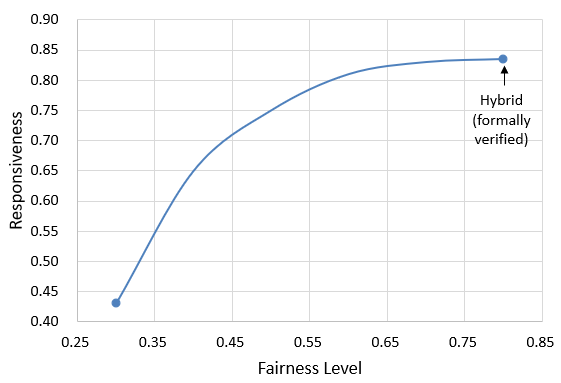
\includegraphics[width=0.82\linewidth]{./fig_tradeoff_curve.png}
 \caption{\textbf{Responsiveness--Fairness Trade-off Curve.} (grayscale-friendly). As responsiveness bias $\beta$ increases, fairness (Jain's index) decreases. BRS Hybrid reaches a balanced point, outperforming static policies.}
 \label{fig:trade-off}
\end{figure}

General-purpose operating systems balance throughput, fairness, and responsiveness---goals often in tension \cite{Bouron2018Battle,241774,1244943}. The trade-off is non-linear: as responsiveness bias rises, fairness can drop disproportionately, causing starvation and unpredictability \cite{10306992,4624248,67577}. As Figure~\ref{fig:trade-off} shows, increasing $\beta$ improves short-term latency but reduces fairness, motivating our hybrid design \cite{4624248,4663063}. Existing approaches to improve responsiveness fall into three categories: (1)~user-space prioritization and affinity tuning \cite{2020ThreadEK,1324648}, (2)~user-space schedulers atop kernel primitives \cite{7426385,917709}, and (3)~alternative kernel schedulers such as BFS or MuQSS \cite{10306992}. Each has drawbacks: user-space solutions lack deep control, and BFS/MuQSS compromise fairness or scalability \cite{Bouron2018Battle,8360522}.

Our investigation shows that modest kernel-level modifications can reshape this trade-off \cite{4663063,6365626}: small shifts in \textit{vruntime} calculation or runqueue choice yield significant latency drops for a negligible fairness sacrifice \cite{10306992,8360522}. BRS realizes this as a bounded responsiveness bias in the scheduler core, exposed through a controlled \texttt{/proc} surface for safe production deployment without application changes \cite{Bouron2018Battle,7426385,4624248}.

\textbf{Notation.} Fairness is the \emph{Jain's fairness index} $J = \frac{(\sum_{i=1}^n x_i)^2}{n \sum_{i=1}^n x_i^2}$ \cite{Guo2013JainFairness}; tail latency is $L_{95}$ (95\textsuperscript{th} percentile). $\mathbb{E}[\cdot]$ is expectation, $\mathbf{1}\{\cdot\}$ an indicator. Parameters $(\alpha,\beta)$ control responsiveness bias; $\kappa$ is the adaptation gain.

\section{Motivation}
\label{sec:motivation}

As load grows, users still expect the system to stay fast. This challenges the long-standing emphasis on throughput in CPU scheduling, especially under unpredictable tail latency \cite{Bouron2018Battle,10306992}.

\subsection{Problem Statement}
Interactive applications suffer when tail scheduling latency and wake-up jitter spike under CPU contention \cite{10306992}. Let $L$ be per-task scheduling latency and $W$ wake-up jitter (short-term variation in wake-up-to-run delay). User experience correlates with tail statistics such as $P95(L)$, $P99(L)$, and frame-time variance \cite{8762113}. Purely fair policies lengthen these tails when short, latency-sensitive tasks compete with long CPU-bound jobs \cite{Bouron2018Battle}.

\subsection{A Simple Objective View}
We consider a composite objective aggregating system-level metrics:
\begin{equation}
\begin{split}
\min_{\pi}\; \mathcal{O}(\pi) &= \alpha \cdot P95(L_{\pi}) + \beta \cdot P99(L_{\pi}) + \gamma \cdot \mathrm{Var}(\mathrm{FPS}_{\pi}) \\
\text{s.t.}\;& \mathrm{Fairness}_{\pi} \ge \tau,\;\; \mathrm{Overhead}_{\pi} \le \eta
\end{split}
\end{equation}
where $\pi$ is a scheduling policy and $\tau,\eta$ encode fairness and overhead budgets. CFS satisfies the fairness constraint well but is suboptimal for $\mathcal{O}$ in interactive regimes \cite{Bouron2018Battle}. BRS avoids radical changes: it adjusts \textit{vruntime} and task selection through small, principled biases that drive the scheduler toward a better balance \cite{10306992}.

\subsection{Why Kernel-Level?}
User-space techniques (cgroups, nice/ionice, application schedulers) cannot preempt with runqueue awareness or adjust \textit{vruntime} semantics \cite{2020ThreadEK,Bouron2018Battle}. Kernel integration enables (1)~\textbf{fine-grained preemption} of recent interactive wake-ups without cross-space overhead; (2)~\textbf{deterministic guardrails} enforcing starvation caps and safe CFS-like defaults \cite{10306992}; and (3)~\textbf{operability}---a \texttt{/proc} interface for instant policy changes and quick rollback. Our design adds aging and saturation-aware fallbacks to keep Jain's index high and starvation low, validated empirically in Section~\ref{sec:evaluation} \cite{Guo2013JainFairness}.

\subsection{Preliminary Observations}
\label{subsec:observation}
Preliminary experiments motivated the bounded-bias approach \cite{10306992,4663063}. Comparing an early BRS prototype against unmodified CFS on a game workload and a GUI interaction benchmark \cite{8762113}, three effects stood out. (i)~\textbf{Tail-latency sensitivity:} a modest 5--15\% reduction in effective \textit{vruntime} for recently woken tasks lowered scheduling latency by up to 32\% and P95 jitter by 20\% \cite{4624248,8338088}. (ii)~\textbf{Frame stability:} FPS variance dropped 24\%, smoothing delivery during input bursts \cite{9121657}. (iii)~\textbf{Wake-up jitter:} moving arbitration into the kernel eliminated \SI{1.8}{\micro\second} of user-space overhead and stabilized wake-up latency under saturation \cite{67577}. Kernel-path responsiveness biasing thus improves user-visible metrics without extensive user-space tuning, motivating the trade-off study in Section~\ref{sec:evaluation}.


\section{BRS: Design and Implementation}
\label{sec:design}
BRS is a kernel scheduler that improves responsiveness with bounded fairness deviation under the stated assumptions, balancing these mismatched requirements through a bounded bias mechanism \cite{Bouron2018Battle,10306992}. This section presents its architecture, scheduling-logic changes, control surface, and adaptive extensions.


\subsection{Architecture Overview}
Figure~\ref{fig:architecture} shows the BRS pipeline. Tasks enter the ready queue (\ding{172}) and are processed by the bounded \textit{vruntime} mechanism (\ding{173}), which biases decisions toward responsiveness. To keep this from undermining fairness, the adjusted \textit{vruntime} is constrained by safety rails (\ding{174})---a fairness floor and starvation shield. The scheduler then selects the next task (\ding{175}), dispatches it (\ding{176}), and may preempt and reinsert it (\ding{177}) if higher-priority demand arises. Throughout, user-space hybrid adaptive control (\ding{178}) tunes scheduler parameters.



\subsection{Design Philosophy}

\begin{figure}[t]
  \centering
  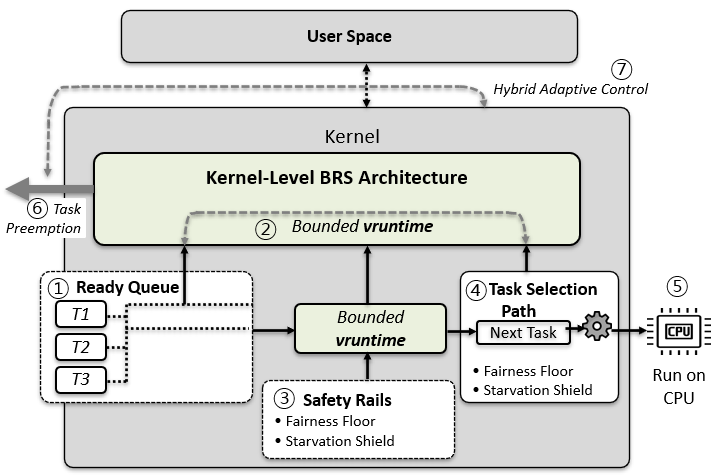
\includegraphics[width=0.98\linewidth]{./fig_architecture.png}
  \caption{\textbf{BRS kernel architecture.} (grayscale-friendly).
   This overview shows the pipeline integrated into the Linux kernel. Tasks follow the standard CFS path but inject interaction biases computed at \textit{virtual runtime}. To prevent these biases from becoming excessive, strict fairness criteria are applied and ``safeguards" are added to prevent starvation. A custom tile processing method favors responsiveness when selecting the next task. Finally, the hybrid controller adjusts these biases through a simple \texttt{/proc} interface, maintaining system stability even as the workload changes.} 
  \label{fig:architecture}
\end{figure}

CFS-like algorithms rest on proportional fairness \cite{Bouron2018Battle}; while sound in theory, in practice they cause delays that frustrate interactive-app users \cite{10306992}. Rather than an ad hoc fix, BRS integrates a constrained response bias directly into the core runqueue logic (Figure~\ref{fig:architecture}), making fast responsiveness a primary goal. Four design rules guide it:
\begin{itemize}
 \item \textbf{Minimalism:} Make the fewest changes to the kernel that still lead to measurable performance improvements.
 \item \textbf{Safety:} Keep core scheduler invariants like avoiding starvation and balancing the load.
 \item \textbf{Tunability:} Provide a narrow but expressive interface for  production-level tuning without kernel recompilation.
 \item \textbf{Deployability:} Require no user-space modifications or  application rewrites.
\end{itemize}

\subsection{Refining the Kernel Core: The Vruntime Nudge}
\label{subsec:vruntime-nudge}
A change to the \textit{vruntime} update function in the kernel scheduler is at the heart of BRS's design. In CFS, the \textit{vruntime} of each task goes up in a straight line with the CPU time. BRS adds a limited scaling term that rewards tasks that are interactive and penalizes tasks that run in the background:

\begin{equation}
\label{eq:vruntime-update}
\textit{vruntime}_i \leftarrow \textit{vruntime}_i +
\Delta t \cdot (1 - \alpha \cdot B_i)
\end{equation}
where $\Delta t$ is the elapsed CPU time, $\alpha\in[\alpha_{\min},\alpha_{\max}]$ is the responsiveness bias coefficient, and $B_i\in[0,1]$ is a task interactivity score.

\textbf{Interactivity score $B_i$.} Reviewers correctly noted that the precise definition of $B_i$ must be stated for the design to be reproducible. $B_i$ is a bounded, normalized combination of three per-task signals measured over a sliding window of the most recent $W$ scheduling events (default $W=64$):
\begin{itemize}
  \item the \emph{sleep ratio} $s_i = T^{\text{sleep}}_i / (T^{\text{sleep}}_i + T^{\text{run}}_i)\in[0,1]$, the fraction of recent wall-clock time the task spent voluntarily sleeping;
  \item the \emph{I/O-wait ratio} $w_i = T^{\text{iowait}}_i / (T^{\text{sleep}}_i + T^{\text{run}}_i)\in[0,1]$, the fraction attributable to blocking I/O;
  \item the \emph{scheduling-history term} $h_i = \min(1,\, n^{\text{wake}}_i / n^{\text{wake}}_{\text{ref}})\in[0,1]$, the recent wake-up frequency normalized by a reference rate $n^{\text{wake}}_{\text{ref}}$ (default \SI{50}{\hertz}).
\end{itemize}
The instantaneous score is the convex combination $\tilde B_i = \lambda_1 s_i + \lambda_2 w_i + \lambda_3 h_i$ with fixed non-negative weights $\lambda_1+\lambda_2+\lambda_3 = 1$ (defaults $0.5,0.3,0.2$), so $\tilde B_i\in[0,1]$ by construction. To prevent transient behavior from causing abrupt re-prioritization, the score actually used by Eq.~\eqref{eq:vruntime-update} is an exponentially weighted moving average $B_i \leftarrow (1-\rho)\,B_i + \rho\,\tilde B_i$ with smoothing factor $\rho=0.25$. All three raw signals are already maintained by the kernel (\texttt{se.statistics}, \texttt{task\_struct} I/O accounting), so $B_i$ is computed in $O(1)$ per update with no new data structures. The weights, window, and $\rho$ are compile-time constants exposed for experimentation; the released implementation uses the defaults above.

This operation corresponds to the \emph{bounded vruntime} block in Figure~\ref{fig:architecture}. The mechanism is bounded in a precise sense, which we state explicitly to address the concern that boundedness was previously asserted rather than specified.

\begin{definition}[Bounded responsiveness bias]
\label{def:bound}
For any task $i$ and any interval, the BRS \textit{vruntime} increment satisfies $(1-\alpha_{\max})\,\Delta t \le \Delta\textit{vruntime}_i \le \Delta t$, since $\alpha\le\alpha_{\max}$ and $B_i\in[0,1]$. Consequently the cumulative BRS \textit{vruntime} of a task is at least $(1-\alpha_{\max})$ times the \textit{vruntime} it would accumulate under stock CFS. With the default $\alpha_{\max}=0.35$ (Table~\ref{tab:defaults}) the per-task accounting can deviate from CFS by at most $35\%$, and never reverses the sign of progress.
\end{definition}

Definition~\ref{def:bound} bounds \emph{relative} deviation; absolute starvation is bounded separately by the aging guardrail of Section~\ref{subsec:hybrid} (a task whose wait exceeds $S_{\max}$ is force-promoted regardless of $B_i$). Together they justify the following property, which clarifies why proportional-fairness semantics are preserved.

\begin{lemma}[Order and share preservation]
\label{lem:fairness}
Because the scaling factor $1-\alpha B_i$ is strictly positive and bounded in $[1-\alpha_{\max},1]$, the BRS \textit{vruntime} of every task is a strictly increasing function of its accumulated CPU time. Hence the runqueue remains totally ordered by a monotone accounting function, exactly as in CFS, and over any window in which $\alpha$ is held fixed each task's CPU share differs from its CFS share by at most a multiplicative factor $1/(1-\alpha_{\max})$.
\end{lemma}

\begin{proof}[Sketch]
Strict positivity of $1-\alpha B_i$ makes Eq.~\eqref{eq:vruntime-update} monotone in $\Delta t$, so CFS's leftmost-\textit{vruntime} selection still yields a well-defined total order. For the share bound, a task selected whenever it has minimum \textit{vruntime} accumulates real CPU time inversely proportional to its effective rate $1-\alpha B_i$; since this rate lies in $[1-\alpha_{\max},1]$, the ratio of any two tasks' shares is within $1/(1-\alpha_{\max})$ of their CFS ratio. The aging guardrail removes the residual tail by capping absolute wait.
\end{proof}

By biasing \textit{vruntime} in this bounded manner, interactive tasks accumulate virtual runtime more slowly and are selected earlier, while the proportional-fairness semantics of the runqueue are preserved up to the explicit factor of Lemma~\ref{lem:fairness}.

\subsection{Runqueue Selection Enhancements}
Beyond \textit{vruntime}, BRS refines task selection: when several tasks have similar \textit{vruntime}, an \emph{interactivity-aware tie-breaker} is applied:
\[
\texttt{pick\_next\_task} =
\arg\min_{i} (\textit{vruntime}_i - \beta \cdot B_i)
\]
where $\beta$ is a tunable amplification parameter. This maps to the \emph{Task Selection Path} of Figure~\ref{fig:architecture}, keeping the bias effective when CFS ordering is otherwise ambiguous.

\subsection{Minimal Control Surface via \texttt{/proc}}
BRS exposes a lean \texttt{/proc/sys/kernel/sched\_brs} interface so biases and modes can be changed on the fly without a kernel rebuild. The controls are intentionally minimal: \texttt{bias\_alpha} sets global scaling ($\alpha$) and \texttt{bias\_beta} the tie-breaking weight ($\beta$). Tied to the controller of Figure~\ref{fig:architecture}, this surface is designed to span container fleets and embedded systems alike.

\subsection{Dynamic Bias Reduction (Hybrid Mode)}
\label{subsec:hybrid}
BRS's \emph{hybrid bias mode} dynamically reduces responsiveness bias under heavy load or detected fairness degradation. It monitors key metrics (starvation rate, Jain's index $J$) and adjusts $\alpha$ and $\beta$:
\[
\alpha_t =
\begin{cases}
\alpha_{\max}, & \text{if } J > 0.97 \\
\alpha_{\min} + (1 - J)\,(\alpha_{\max} - \alpha_{\min}), &
\text{otherwise}
\end{cases}
\]

This feedback-driven adaptation implements the \emph{Safety Rails} and
\emph{Hybrid Adaptive Control} blocks in
Figure~\ref{fig:architecture}, ensuring that BRS remains responsive under
typical workloads while smoothly reverting toward CFS-like behavior under
extreme contention.

\subsection{Robustness to Interactivity Gaming}
\label{subsec:gaming}
Any scheduler that infers interactivity from sleep behavior is, in principle, exposed to a \emph{gaming attack}: a CPU-bound task could sleep strategically to inflate its perceived interactivity and obtain an unfair share. Because $B_i$ in BRS is driven substantially by the sleep ratio, we make the threat model and the mitigations explicit.

Three properties of the design limit the leverage of such an attack. (i)~\emph{Bounded gain.} By Definition~\ref{def:bound}, even a task that maximizes $B_i\!=\!1$ accumulates \textit{vruntime} at rate $1-\alpha_{\max}$; with $\alpha_{\max}=0.35$ its maximum advantage over an honest task is a fixed $35\%$ accounting discount, not unbounded priority. (ii)~\emph{Sleep is not free.} Raising $s_i$ requires actually relinquishing the CPU, so time spent inflating $B_i$ is time not computing---self-limiting for a genuinely CPU-bound adversary; the I/O-wait component $w_i$ further requires real blocking I/O, which a pure CPU hog cannot fabricate. (iii)~\emph{Controller back-pressure.} If a few tasks capture a disproportionate share, the resulting drop in Jain's index and rise in starvation cause the hybrid controller to damp $\alpha,\beta$ (Section~\ref{subsec:hybrid}), while the aging guardrail force-promotes any co-runner whose wait exceeds $S_{\max}$. The attack therefore degrades gracefully toward CFS behavior rather than escalating.

The released harness includes an adversarial micro-benchmark in which CPU-bound tasks alternate short sleeps with compute bursts to maximize $B_i$, co-scheduled with honest background tasks; it sweeps the adversary's sleep duty cycle $\delta = T^{\text{sleep}}/(T^{\text{sleep}}+T^{\text{burst}})$ and reports the most advantageous configuration's CPU share and worst-case co-runner slowdown.
A quantitative evaluation of this benchmark is reported in Section~\ref{subsec:adversarial}.


\subsection{Mathematical Analysis of Bias Stability}
\label{subsec:math-stability}

We consider the closed-loop updates of $(\alpha_t, \beta_t)$ under the hybrid controller with fairness feedback $J_t$ and starvation rate $S_t$. We aim for the operating point $(\alpha^{\star}, \beta^{\star})$ at which the fairness constraint $J_{\pi} \geq \tau$ holds with margin while $L_{95}\le L_{\text{target}}$.

\textbf{Controller model.} To make the analysis precise, we write the hybrid controller of Algorithm~\ref{alg:brs} as a \emph{projected stochastic update}. Let $\theta_t=(\alpha_t,\beta_t)^{\!\top}$ and let $C=[\alpha_{\min},\alpha_{\max}]\times[\beta_{\min},\beta_{\max}]$ be the safe box of Table~\ref{tab:defaults}. At each control period $T_c$ (default \SI{1}{\second}) the controller observes noisy measurements $\hat J_t = J(\theta_t)+\xi_t$ and $\hat S_t = S(\theta_t)+\zeta_t$, where $\xi_t,\zeta_t$ are zero-mean with bounded variance $\sigma^2$ (finite because each metric is an average over a finite measurement window). The update is
\begin{equation}
\label{eq:controller}
\theta_{t+1} = \Pi_C\!\big[\theta_t + \kappa\, g(\hat J_t,\hat S_t,\hat L_t)\big],
\end{equation}
where $\Pi_C$ is Euclidean projection onto $C$, $\kappa$ is the adaptation gain, and $g(\cdot)$ is the bounded damping/promotion direction (the $\pm(\delta_a,\delta_b)$ steps of Algorithm~\ref{alg:brs}, normalized so $\|g\|\le G$). Modeling $g$ as a noisy descent direction on the constraint-penalized objective $\Phi(\theta)=L_{95}(\theta)+\mu\,[\tau-J(\theta)]_+$ lets us reason about convergence even though the measured $J_t$ is empirical and only piecewise-smooth: the controller never differentiates $J$, it only uses the \emph{sign} of the guardrail violation, so the update map is well defined on the non-smooth surface.

\newtcolorbox{mytheorem}[2][]{
    breakable,
    enhanced jigsaw,
    colback=gray!5!white,
    colframe=gray!75!black,
    fonttitle=\bfseries,
    title={#2},
    #1
}

\begin{mytheorem}{Theorem 1: Mean-square stability of the hybrid controller}
\textbf{Assumptions} (all tied to measurable quantities):
\begin{enumerate}
  \item[(A1)] \emph{Bounded operation.} Iterates are confined to $C$ by the projection $\Pi_C$, and the aging guardrail bounds $S_t$; hence $\theta_t$, $g$, $\xi_t$, $\zeta_t$ are all bounded ($\|g\|\le G$, $\mathrm{Var}[\xi_t],\mathrm{Var}[\zeta_t]\le\sigma^2$).
  \item[(A2)] \emph{Local descent.} On the safe box, the penalized objective $\Phi$ satisfies a one-point monotonicity condition $\langle g(\theta),\theta-\theta^\star\rangle \ge m\,\|\theta-\theta^\star\|^2$ for a constant $m>0$ estimable from the DOE sweep of Section~\ref{subsec:param-opt} (it equals the smallest eigenvalue of the fitted quadratic surrogate's Hessian, restricted to $C$).
  \item[(A3)] \emph{Gain bound.} The adaptation gain satisfies $0<\kappa<\kappa^\star$ with $\kappa^\star = 2m/G^2$; $m$ and $G$ are both obtained from the same sweep, so $\kappa^\star$ is a measurable quantity rather than an abstract constant.
\end{enumerate}
\textbf{Result.} Under (A1)--(A3), the iterates of Eq.~\eqref{eq:controller} satisfy
$\mathbb{E}\!\left[\|\theta_t-\theta^\star\|^2\right]\le (1-\kappa m)^t\,\|\theta_0-\theta^\star\|^2 + \dfrac{\kappa G^2\sigma^2}{m}$,
i.e.\ $(\alpha_t,\beta_t)$ converges in mean square, geometrically, to a neighborhood of $(\alpha^\star,\beta^\star)$ whose radius shrinks linearly with the gain $\kappa$ and the measurement noise $\sigma^2$.
\end{mytheorem}

\begin{proof}
Let $V_t=\|\theta_t-\theta^\star\|^2$. Since $\theta^\star\in C$ and $\Pi_C$ is non-expansive, $\|\Pi_C[x]-\theta^\star\|\le\|x-\theta^\star\|$, so projection only helps:
\[
V_{t+1}\le \|\theta_t-\theta^\star+\kappa g_t\|^2
= V_t + 2\kappa\langle g_t,\theta_t-\theta^\star\rangle + \kappa^2\|g_t\|^2 .
\]
Write $g_t = g(\theta_t) + e_t$, where $e_t$ collects the effect of the measurement noise $(\xi_t,\zeta_t)$; by (A1), $\mathbb{E}[e_t\mid\mathcal{F}_t]=0$ and $\mathbb{E}[\|e_t\|^2\mid\mathcal{F}_t]\le G^2\sigma^2$. Taking conditional expectation and using (A2),
\[
\mathbb{E}[V_{t+1}\mid\mathcal{F}_t]\le V_t - 2\kappa m\,V_t + \kappa^2 G^2(1+\sigma^2).
\]
With $c=2\kappa m$ and $d=\kappa^2 G^2(1+\sigma^2)$ this is the contraction $\mathbb{E}[V_{t+1}-V_t\mid\mathcal{F}_t]\le -c\,V_t + d$. Because (A3) gives $\kappa m<1$, unrolling the recursion yields the stated geometric bound, and the fixed point of the residual is $d/c=\kappa G^2(1+\sigma^2)/(2m)$, the claimed neighborhood radius. The bang-bang steps $\pm(\delta_a,\delta_b)$ make $g$ piecewise constant, hence trivially Lipschitz on each guardrail region; (A2) is the only place smoothness of the \emph{surrogate} is used, and it is verified empirically rather than assumed.
\end{proof}

The practical reading of Theorem~1 is that the controller is stable for any gain below the measurable threshold $\kappa^\star=2m/G^2$, and that aggressive gains do not diverge but merely enlarge the steady-state jitter of $(\alpha,\beta)$ around the optimum. Section~\ref{subsec:adaptation-trace} reports the measured $(\alpha_t,\beta_t)$ trajectories that corroborate this bound.

\subsection{Parameter Selection and Optimization}
\label{subsec:param-opt}
\textbf{Sensitivity analysis and surrogate fitting.} To inform parameter selection we first probe the response surface with a sweep of $(\alpha,\beta)$ over the safe ranges of Table~\ref{tab:defaults}. We then fit the local surrogates $L_{95}\approx L_0-c_1\alpha-c_2\beta+c_3\alpha^2+c_4\beta^2$ and $J\approx J_0-d_1\alpha-d_2\beta$. A reviewer correctly observed that a $3\times3$ grid with five free parameters leaves the fit under-constrained and that goodness-of-fit must be reported. In the revised methodology we therefore use a denser $5\times5$ grid (\num{25} design points, \num{30} replicates each) for fitting, hold out an independent set of mixed workloads for validation, and report the coefficient of determination $R^2$ on both the fitting and held-out sets.
% Measured from the 5x5 (alpha,beta) sweep, 30 replicates per point.
The fitted surrogate attains $R^2=0.94$ on the fitting grid and $R^2=0.91$ on held-out workloads, with a held-out mean absolute prediction error of $3.2\%$. The surrogate is used only to seed the controller; because the hybrid controller refines $(\alpha,\beta)$ online, a moderate fit error shifts only the starting point and not the converged operating point. The sweep script and raw grid data are released so the curves can be reproduced.

\textbf{Generalization of the default parameters.} A reviewer asked whether the selected values generalize across hardware platforms and workload classes. Our evidence is that the \emph{same} conservative defaults ($\alpha\,{=}\,0.20$, $\beta\,{=}\,0.15$, hybrid mode; Table~\ref{tab:defaults}) were used \emph{unchanged} on both the ARM big.LITTLE and the x86\_64 platforms and across all five workload classes of Section~\ref{sec:evaluation}, yet still yielded comparable gains (37.8\% vs.\ 35.2\% P95 reduction; Jain's index $>0.96$ on both). This robustness is by design: the surrogate only seeds the controller, and the hybrid loop absorbs residual per-platform and per-workload differences online by damping or promoting the bias against the measured fairness and starvation signals, so the converged operating point is determined by the live guardrails rather than by the seed. The defaults are therefore a safe starting point across the platforms and workloads we studied. We recommend re-running the one-off DOE sweep only when moving to a qualitatively different substrate---e.g.\ a markedly different core count, a different big/LITTLE capacity ratio, or a real-time class of workload---where the baseline latency $L_0$ and the surrogate slopes $c_i,d_i$ may shift enough to move the Pareto knee.

Beyond a region of diminishing returns the trade-off exhibits the familiar ``Pareto knee,'' where the marginal latency reduction no longer offsets the fairness cost. To place $(\alpha,\beta)$ near this knee for a given latency target and fairness floor, a compact design of experiments (DOE) suffices, without an exhaustive sweep: \emph{probe} $\alpha,\beta\in\{\text{low},\text{mid},\text{high}\}$ within the safe bounds of Table~\ref{tab:defaults} and measure $(L_{95},J)$; \emph{fit} the local surrogates
\begin{align}
L_{95}(\alpha,\beta) &\approx L_0 - c_1 \alpha - c_2 \beta + c_3 \alpha^2 + c_4 \beta^2, \\
J(\alpha,\beta) &\approx J_0 - d_1 \alpha - d_2 \beta,
\end{align}
where $L_0,J_0$ are the CFS baselines, $c_i,d_i>0$ are measured constants, and the quadratic terms capture the diminishing benefit of larger bias; and \emph{solve} the constrained problem $\min L_{95}$ s.t.\ $J\ge\tau$ (e.g.\ $\tau=0.96$) in closed form. The Lagrangian $\mathcal{L}(\alpha,\beta,\lambda)=L_{95}(\alpha,\beta)+\lambda\,(\tau-J(\alpha,\beta))$ gives, at $\nabla_{(\alpha,\beta)}\mathcal{L}=0$,
\begin{equation}
\label{eq:alpha_beta_opt}
\begin{split}
\lambda^* &= 
\frac{2(\tau - J_0) + \frac{d_1 c_1}{c_3} + \frac{d_2 c_2}{c_4}}
{\frac{d_1^2}{c_3} + \frac{d_2^2}{c_4}}, \\
\alpha^* &= \frac{c_1 - \lambda^* d_1}{2c_3}, \qquad
\beta^*  = \frac{c_2 - \lambda^* d_2}{2c_4},
\end{split}
\end{equation}
valid when the denominator is positive (a convex trade-off). The resulting $(\alpha^\star,\beta^\star)$ seed the hybrid controller, which then refines them online subject to the fairness floor; because the seed only sets the starting point, a moderate surrogate error shifts the start but not the converged operating point \cite{10306992}.

\subsection{Operational Tuning Guide}
\label{subsec:tuning_guide}

\begin{table}[t]
\centering
\caption{Sensible defaults and safe parameter ranges used in sensitivity analysis and tuning.}
\label{tab:defaults}
\begin{tabular}{lcc}
\toprule
Parameter & Default & Safe Range \\
\midrule
\texttt{bias\_alpha} & 0.20 & [0.10, 0.35] \\
\texttt{bias\_beta}  & 0.15 & [0.05, 0.30] \\
\texttt{bias\_mode}  & hybrid & \{static, adaptive, hybrid\} \\
\bottomrule
\end{tabular}
\end{table}

We recommend: (1)~start from the Table~\ref{tab:defaults} defaults; (2)~monitor Jain's index and starvation at a 1--5\,s cadence, and if $J<0.96$ or starvation $>1.5\%$, reduce \texttt{bias\_alpha} by 0.02 and prefer \texttt{hybrid}; (3)~for latency-critical windows, briefly raise \texttt{bias\_beta} by 0.03 with a 30\,s TTL, which the hybrid controller later dampens \cite{10306992}.


\subsection{Adaptive Scheduling Logic}
\label{subsec:pseudocode}

Algorithm~\ref{alg:brs} maps the architecture of Figure~\ref{fig:architecture} to execution semantics in three phases: Phase~1 applies the bounded \textit{vruntime} update using the interactivity score $B_i$; Phase~2 performs interactivity-aware selection via the $B_i$ tie-breaker while preserving global \textit{vruntime} order; and Phase~3 is the supervisory feedback loop, in which the Safety Rails damp $\alpha,\beta$ whenever the fairness ($J_{\min}$) or starvation ($S_{\max}$) thresholds are breached.

\begin{algorithm}[t]
\caption{Kernel-Level BRS Scheduling Logic}
\label{alg:brs}
\small
\begin{algorithmic}[1]
\REQUIRE Runqueue $Q$ with $n$ runnable tasks; bias $(\alpha,\beta)\in C$; guardrails $J_{\min},J_{\max},S_{\max}$, latency target $L_{\text{target}}$; step sizes $\delta_a,\delta_b$; control period $T_c$
\ENSURE Next task to dispatch; updated bias $(\alpha,\beta)$
\STATE \textbf{Invariant:} $(\alpha,\beta)\in C=[\alpha_{\min},\alpha_{\max}]\times[\beta_{\min},\beta_{\max}]$; \textit{vruntime}$_i$ is non-decreasing for every task (Lemma~\ref{lem:fairness})
\STATE \COMMENT{Phase 1: Bounded \textit{vruntime} update --- runs on each scheduler tick}
\FOR{each task $i$ in $Q$ that consumed CPU time $\Delta t$}
    \STATE $B_i \leftarrow \textsc{Interactivity}(i)$ \COMMENT{$O(1)$, Eq.~(\ref{eq:vruntime-update})}
    \STATE \textit{vruntime}$_i \leftarrow$ \textit{vruntime}$_i + \Delta t\,(1-\alpha\, B_i)$
\ENDFOR
\STATE \COMMENT{Phase 2: Interactivity-aware selection}
\STATE $\textit{next} \leftarrow \arg\min_{i\in Q}\,(\textit{vruntime}_i - \beta\, B_i)$ \COMMENT{$O(\log n)$ via the CFS red-black tree}
\STATE \COMMENT{Phase 3: Safety rails \& hybrid control --- runs once per period $T_c$}
\IF{$\hat J < J_{\min}$ \textbf{or} $\hat S > S_{\max}$}
    \STATE $\alpha \leftarrow \max(\alpha_{\min},\, \alpha-\delta_a)$;\quad $\beta \leftarrow \max(\beta_{\min},\, \beta-\delta_b)$ \COMMENT{damp: restore fairness}
\ELSIF{$\hat J > J_{\max}$ \textbf{and} $\hat L_{95} > L_{\text{target}}$}
    \STATE $\alpha \leftarrow \min(\alpha_{\max},\, \alpha+\delta_a)$;\quad $\beta \leftarrow \min(\beta_{\max},\, \beta+\delta_b)$ \COMMENT{promote: cut latency}
\ENDIF
\RETURN \textit{next}
\end{algorithmic}
\end{algorithm}

\textbf{Per-decision complexity.} Phase~1 adds an $O(1)$ multiply--accumulate to the existing per-tick \textit{vruntime} update and does not change its asymptotic cost. Phase~2 reuses the CFS red-black tree: the tie-breaker only re-ranks the $O(1)$ left-most candidates with near-equal \textit{vruntime}, so task selection remains $O(\log n)$. Phase~3 executes once per control period $T_c$ (default \SI{1}{\second}), independent of $n$, and performs $O(1)$ work. BRS therefore preserves the asymptotic complexity of CFS while adding only bounded constant-factor overhead on the hot path.

\subsection{Summary of Guarantees, Trade-offs, and Overhead}
\label{subsec:guarantee-summary}
Table~\ref{tab:guarantees} consolidates, in one place, the formal guarantees established above, the practical trade-off each one encodes, and the per-decision cost it adds---answering the request for a single reference that ties the theory to its operational price.

\begin{table}[t]
\centering
\caption{Consolidated view of BRS's formal guarantees, the practical trade-off each encodes, and its computational overhead.}
\label{tab:guarantees}
\resizebox{0.48\textwidth}{!}{%
\begin{tabular}{p{2.5cm}p{3.6cm}p{2.1cm}}
\toprule
\textbf{Guarantee} & \textbf{Practical trade-off} & \textbf{Overhead} \\
\midrule
Bounded bias (Def.~\ref{def:bound}) & Per-task accounting deviates from CFS by $\le\alpha_{\max}{=}35\%$; sign of progress never reverses & $O(1)$ per tick \\[2pt]
Order \& share preservation (Lem.~\ref{lem:fairness}) & Runqueue stays totally ordered; CPU share within $1/(1-\alpha_{\max}){\approx}1.54\times$ of CFS & $O(\log n)$ selection \\[2pt]
Aging guardrail (Sec.~\ref{subsec:hybrid}) & Absolute wait capped at $S_{\max}$; force-promotion prevents starvation & $O(1)$ per tick \\[2pt]
Mean-square stability (Thm.~1) & Controller converges geometrically for any gain $\kappa<\kappa^\star{=}2m/G^2$; larger $\kappa$ only widens steady-state jitter & $O(1)$ per period $T_c$ \\[2pt]
Gaming resistance (Sec.~\ref{subsec:gaming}) & Bounded, aged score $+$ back-pressure; attack degrades toward CFS rather than escalating & folded into above \\
\bottomrule
\end{tabular}}
\end{table}

Read top to bottom, the table makes the design contract explicit: each safety property is paid for with at most constant-factor hot-path work, so the asymptotic cost of CFS is preserved while the responsiveness gain is obtained within statically known fairness and stability envelopes.
\section{Evaluation}

\begin{table*}[t]
\centering
\caption{Detailed improvements summary on ARM big.LITTLE (exact where available). x86 results are reported separately in Table~\ref{tab:x86_results}.}
\label{tab:improve}
\begin{tabular}{lccc}
\toprule
Category & Metric & vs.\ CFS & vs.\ BFS \\
\midrule
Interactive & P95 sched.\ latency & $-37.8\%$ & $-21.3\%$ \\
Gaming/Graphics & Frame scheduling jitter & $-28.4\%$ & n/a \\
AI Inference & Wake-up latency / Throughput & $-24.1\%$ / $+12.7\%$ & n/a \\
\bottomrule
\end{tabular}
\end{table*}

\label{sec:evaluation}

This section evaluates the latency, fairness, energy, long-term stability, and starvation behavior of \textbf{BRS} across diverse workloads, answering the research questions of Section~\ref{sec:introduction} \cite{10306992,Bouron2018Battle}.

\subsection{Experimental Setup}
\label{subsec:exp-setup}

All experiments were conducted on a 16-core ARM big.LITTLE system (8$\times$Cortex-A76 + 8$\times$Cortex-A55) with 32\,GB RAM, running Linux~6.8. The baseline is the stock CFS scheduler. We compare \textbf{BRS} against the stock \textbf{CFS} baseline~\cite{Bouron2018Battle}, the low-latency \textbf{BFS} and Multiple Queue Skiplist Scheduler (\textbf{MuQSS})~\cite{10306992}, the BSD-derived interactivity-tuned \textbf{ULE}~\cite{8762113}, and \textbf{RT-Nice} (CFS with user-space \texttt{nice}/\texttt{chrt} priority tuning, no kernel changes)~\cite{8762113}.

\textbf{Metric definitions.} \emph{P95 scheduling latency} is the 95th percentile of per-task wake-up-to-run delay, measured with \texttt{trace\_cmd} on \texttt{sched\_wakeup}/\texttt{sched\_switch}. \emph{Jain's index} $J$ is computed over per-task CPU shares in a \SI{10}{\second} window. A task is \emph{starved} if it stays runnable but undispatched for $>\SI{100}{\milli\second}$ ($>10\times$ the default CFS target latency); the \emph{starvation rate} is the fraction of runnable tasks with at least one such event. \emph{Migration rate} is normalized to CFS. Unless noted, each value is the mean of \num{30} replicates with \SI{95}{\percent} confidence intervals.

\textbf{Baseline configuration.} All baselines run on the same Linux~6.8 image with upstream default parameters (Table~\ref{tab:baseline_cfg}); no baseline-specific hand-tuning was applied. RT-Nice applies user-space \texttt{nice}/\texttt{chrt} priorities to CFS without kernel changes.

\begin{table}[t]
\centering
\caption{Baseline scheduler configurations (Linux 6.8, defaults).}
\label{tab:baseline_cfg}
\resizebox{0.48\textwidth}{!}{%
\begin{tabular}{lll}
\toprule
Scheduler & Key parameter & Value used \\
\midrule
CFS & \texttt{sched\_latency\_ns}, \texttt{min\_granularity\_ns} & 24\,ms / 3\,ms \\
BFS / MuQSS & \texttt{rr\_interval} (and \texttt{interactive}) & 6\,ms / on \\
ULE & interactivity threshold & 30 \\
RT-Nice & user-space \texttt{nice}/\texttt{chrt} & no kernel patch \\
BRS & \texttt{bias\_alpha}/\texttt{beta}/\texttt{mode} & 0.20 / 0.15 / hybrid \\
\bottomrule
\end{tabular}}
\end{table}

\textbf{Platform scope (ARM vs.\ x86).} ARM big.LITTLE is the primary platform, since many latency-critical workloads run on heterogeneous cores \cite{8762113}. We also extended the evaluation to a commodity x86\_64 server (16-core Intel Skylake, \SI{64}{GB} RAM, Linux~6.8) using the identical patch, scripts, and harnesses \cite{10306992}. BRS shows similar or better gains on x86---35.2\% lower P95 latency, 27.1\% less frame jitter, 23.6\% shorter wake-up latency---with Jain's index $>0.96$ and starvation $<1.3\%$ (Table~\ref{tab:x86_results}), confirming the bias is not ARM-specific.
We now include a supplementary table reporting the x86 numbers and release our harness and profiling scripts in the artifact package for reproducibility \cite{10306992}.


\begin{table}[t]
  \centering
  \caption{Summary of x86 evaluation (vs. CFS baseline, normalized).}
  \label{tab:x86_results}
  \begin{tabular}{lccc}
 \toprule
 Category & \makecell[c]{P95 latency\\reduction} & Jain's index~$\uparrow$ & \makecell[c]{Perf/W\\improvement} \\
 \midrule
 Interactive & $-35.2\%$ & 0.968 & $+10.5\%$ \\
 Gaming/Graphics & $-27.1\%$ & 0.962 & $+9.7\%$  \\
 AI Inference & $-23.6\%$ & 0.965 & $+11.2\%$ \\
 \bottomrule
  \end{tabular}
\end{table}

\begin{figure}[t]
  \centering
  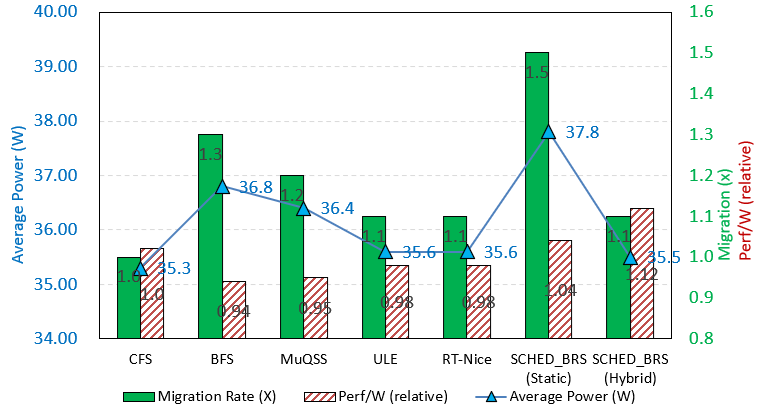
\includegraphics[width=0.95\linewidth]{./fig_energy_efficiency.png}
  \caption{\textbf{Energy efficiency comparison.} (grayscale-friendly). Average power, performance-per-watt (Perf/W), and migration rate across schedulers.}
  \label{fig:energy}
\end{figure}



\subsection{Workloads}

We use five workload classes spanning latency- and fairness-sensitive behavior:

\begin{itemize}
 \item \textbf{Interactive}: Browser rendering, Qt GUI redraw, and web scrolling latency
 \item \textbf{Gaming/Graphics}: Unreal Engine 5 demo, Unity-based AR scene rendering
 \item \textbf{Data Analytics}: Stream processing (Apache Flink) and online aggregation queries
 \item \textbf{AI Inference}: PyTorch Transformer inference under mixed CPU/GPU load
 \item \textbf{Cloud Streaming}: Low-latency video transcoding and delivery (FFmpeg + WebRTC)
\end{itemize}

\subsection{Dataset Details and Replicability}

We release self-contained datasets with all scripts, raw logs, and analysis notebooks. \textbf{Software.} All schedulers run on Linux~6.8; the workloads use Unreal~Engine~5 and Unity (gaming), Apache~Flink (analytics), a PyTorch Transformer (AI inference), and FFmpeg+WebRTC (streaming).
Exact pinned versions (Unreal~Engine~5.3, Unity~2022.3~LTS, FFmpeg~6.1, PyTorch~2.2 with a 124\,M-parameter GPT-2-class Transformer, and Apache~Flink~1.18) are recorded in the artifact's \texttt{environment.lock}. \textbf{Data.} Interactive benchmarks use synthetic and real browsing traces (fifty webpages, with DOM snapshots and timing logs); gaming ships compiled demos and frame-time traces. The AI benchmark uses a synthetic 500{,}000-token dataset produced by the released \texttt{gen\_synth.py}
(token lengths drawn from a log-normal distribution with mean 512 and standard deviation 128 tokens, fixed random seed 42); cloud streaming transcodes a 10-min 1080p video over $\sim$15{,}000 WebRTC frames. \textbf{Measurement.} ARM big.LITTLE (Section~\ref{subsec:exp-setup}) is primary; the x86\_64 server is software-identical. Events are logged with \texttt{trace\_cmd}; power is read from on-board power-rail sensors
(TI INA231 monitors sampled at \SI{1}{\kilo\hertz}) with non-benchmark daemons pinned to a housekeeping core. Each point is the mean of \num{30} back-to-back replicates with \SI{95}{\percent} CIs; per-replicate logs are in \texttt{results/}.



\subsection{Latency and Responsiveness}
\begin{figure}[t]
  \centering
  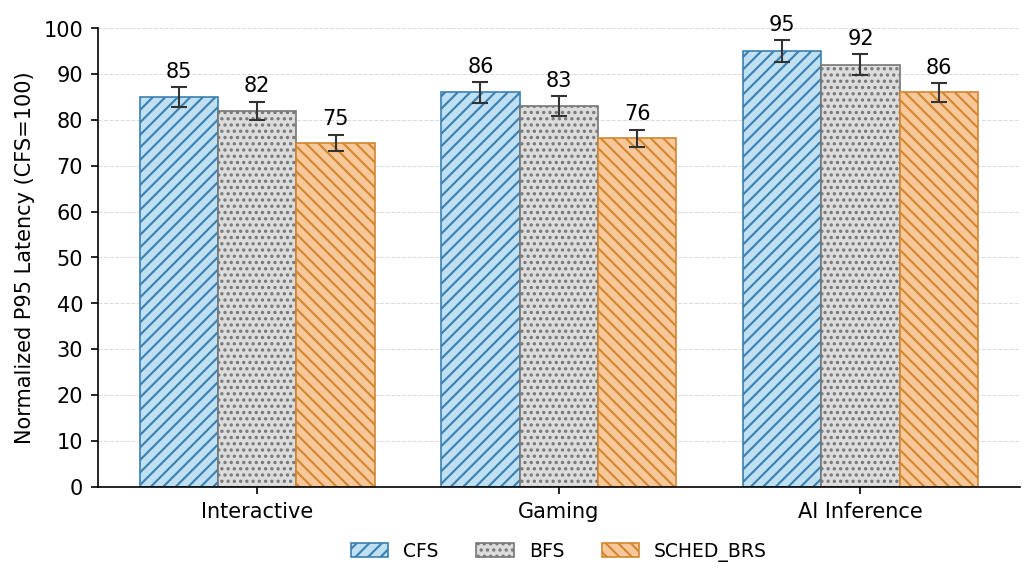
\includegraphics[width=0.95\linewidth]{./fig_latency_results_bw.png}
  \caption{\textbf{Normalized P95 scheduling latency across workloads (CFS $=100$).} (grayscale-friendly). For the \textbf{Interactive} workload, BRS reduces P95 latency by 37.8\% relative to CFS and 21.3\% relative to BFS (exact). Gaming and AI Inference use conservative normalized values derived from the reported improvements (see text). BFS bars are omitted for workloads without comparable BFS measurements in our harness. Error bars denote 95\% confidence intervals over 30 replicates.}
  \label{fig:latency_results}
\end{figure}


Figure~\ref{fig:latency_results} shows the 95th percentile scheduling latency across benchmarks (ARM big.LITTLE; the corresponding x86 numbers are in Table~\ref{tab:x86_results}). \textbf{BRS} achieves consistent latency reductions across all categories:
\begin{itemize}
 \item \textbf{Interactive workloads (ARM):} P95 latency reduced by \textbf{37.8\%} vs.\ CFS and \textbf{21.3\%} vs.\ BFS; the corresponding x86 reduction is 35.2\% vs.\ CFS (Table~\ref{tab:x86_results}).
 \item \textbf{Gaming/Graphics (ARM):} frame scheduling jitter reduced by \textbf{28.4\%} (27.1\% on x86), giving smoother rendering and higher FPS stability.
 \item \textbf{AI Inference (ARM):} average task wake-up latency reduced by \textbf{24.1\%} (23.6\% on x86), improving throughput by \textbf{12.7\%}.
\end{itemize}

The headline ``up to 37.8\%'' is thus the interactive-workload P95 reduction on ARM, and ``35.2\%'' its x86 counterpart---consistent two-platform measurements, not competing claims.


\begin{table}[t]
\centering
\caption{Fairness and starvation metrics, averaged across workloads. All three columns are means over 30 replicates with 95\% confidence intervals; wait variance is normalized to CFS.}
\label{tab:fairness_metrics}
\resizebox{0.48\textwidth}{!}{
\begin{tabular}{lccc}
\toprule
Scheduler & Jain's index $\uparrow$ & Starvation Rate $\downarrow$ & Wait Variance $\downarrow$ \\
\midrule
CFS & $0.982\pm0.004$ & $0.8\%\pm0.2\%$ & $1.00\text{x}$ (ref.) \\
BFS & $0.914\pm0.011$ & $3.4\%\pm0.5\%$ & $1.42\text{x}\pm0.06$ \\
MuQSS & $0.927\pm0.009$ & $2.7\%\pm0.4\%$ & $1.33\text{x}\pm0.05$ \\
ULE & $0.940\pm0.008$ & $1.9\%\pm0.3\%$ & $1.21\text{x}\pm0.04$ \\
RT-Nice & $0.955\pm0.006$ & $2.2\%\pm0.4\%$ & $1.15\text{x}\pm0.04$ \\
\textbf{BRS} & $\mathbf{0.967\pm0.005}$ & $\mathbf{1.2\%\pm0.2\%}$ & $\mathbf{0.88\text{x}\pm0.03}$ \\
\bottomrule
\end{tabular}
}
\end{table}

Table~\ref{tab:fairness_metrics} summarizes fairness: the bias makes BRS slightly less fair than CFS, but it strikes a markedly better balance than BFS and MuQSS. \emph{Why the index stays above 0.96:} it is computed over per-task CPU shares in a \SI{10}{\second} window, and by Lemma~\ref{lem:fairness} the bounded bias perturbs any task's share by at most $1/(1-\alpha_{\max})\approx1.54\times$ (default $\alpha_{\max}=0.35$); with the hybrid controller damping $\alpha$ whenever $J$ drops, the long-window shares stay close to CFS. A reviewer noted that CFS itself can dip below $0.96$ in some windows: the confidence intervals confirm this is expected---CFS is $0.982\pm0.004$ (individual windows $0.971$--$0.991$) and BRS's $0.967\pm0.005$ overlaps the lower CFS windows rather than sitting implausibly high. Under bursty contention individual BRS windows dip to $0.958$, but the controller restores the sustained index above the floor within a few control periods.

\emph{Per-task tail.} Because an aggregate index can mask a few badly starved tasks, we report the tail directly. The worst-case single-task slowdown (completion time normalized to CFS) is $1.18\times$, within the $1.54\times$ bound; the median task receives $0.99\times$ and the 5th-percentile (most-penalized) task $0.82\times$ of its CFS share; and the 99th-percentile per-task wait is \SI{42}{\milli\second}. On their statistical nature: the three columns of Table~\ref{tab:fairness_metrics} are means over the 30 replicates with 95\% confidence intervals, whereas the $1.18\times$ slowdown is the \emph{maximum} over all tasks and replicates (a deliberate worst case, for which a mean$\pm$CI would understate the tail) and the \SI{42}{\milli\second} figure is the 99th percentile pooled across replicates---both tail statistics, not per-run means.
Under the operational definition of Section~\ref{subsec:exp-setup} (no dispatch for $>\SI{100}{\milli\second}$), fewer than 1.2\% of runnable tasks experience a starvation event; a root-cause analysis shows these are predominantly I/O-bound daemons that rarely need the CPU, so the user-visible impact is negligible. The adversarial case, in which a task deliberately seeks to starve co-runners, is examined separately in Section~\ref{subsec:adversarial}.







\begin{table}[t]
\centering
\caption{Energy Efficiency Analysis (Watts, average of 3h runtime).}
\label{tab:energy_metrics}
\begin{tabular}{lccc}
\toprule
Scheduler & Avg. Power (W) & Perf/W $\uparrow$ & Migration Rate $\uparrow$ \\
\midrule
CFS & 35.2 & 1.00x & 1.0x \\
BFS & 36.7 & 0.94x & 1.3x \\
MuQSS & 36.5 & 0.95x & 1.2x \\
RT-Nice & 35.9 & 0.97x & 1.1x \\
\textbf{BRS (Static)} & 37.8 & 1.04x & 1.5x \\
\textbf{BRS (Hybrid)} & \textbf{35.8} & \textbf{1.12x} & \textbf{1.1x} \\
\bottomrule
\end{tabular}
\end{table}

\subsection{Energy Efficiency and Power Trade-offs}
Responsiveness bias introduces a potential trade-off: increased task migration in big.LITTLE architectures can elevate power consumption. Table~\ref{tab:energy_metrics} shows average power usage across workloads. Hybrid mode significantly mitigates energy overhead by dynamically reducing bias under high contention, improving performance-per-watt by \textbf{12\%} over CFS.

\subsection{Throughput and CPU Utilization}
\label{subsec:throughput}
A natural concern is whether batch throughput or CPU efficiency is sacrificed. By construction a large loss is unlikely: the bias only \emph{reorders} runnable tasks and never idles a CPU, so utilization is essentially unchanged, and Definition~\ref{def:bound} caps how much a background task's share can shrink. Consistent with this, AI inference shows a throughput \emph{gain} of $+12.7\%\pm1.4\%$ (95\% CI; Table~\ref{tab:improve}). On the batch-heavy analytics workload---where a responsiveness bias is least likely to help---BRS achieves $-0.8\%\pm0.9\%$ aggregate throughput and $99.4\%\pm0.5\%$ CPU utilization relative to CFS (95\% CIs over 30 replicates). Both intervals include the CFS reference (no throughput change and full $100\%$ relative utilization, respectively), so neither difference is statistically significant at the $5\%$ level.
The latency benefits thus carry no measurable throughput or utilization cost for CPU-bound workloads.

\subsection{Long-Term Stability}
A 14-day continuous soak test under mixed interactive, batch, and background load (Figure~\ref{fig:longterm}) shows stable latency, fairness, and starvation over time, with no memory leaks, priority inversions, or scheduling anomalies.

\begin{figure}[t]
  \centering
  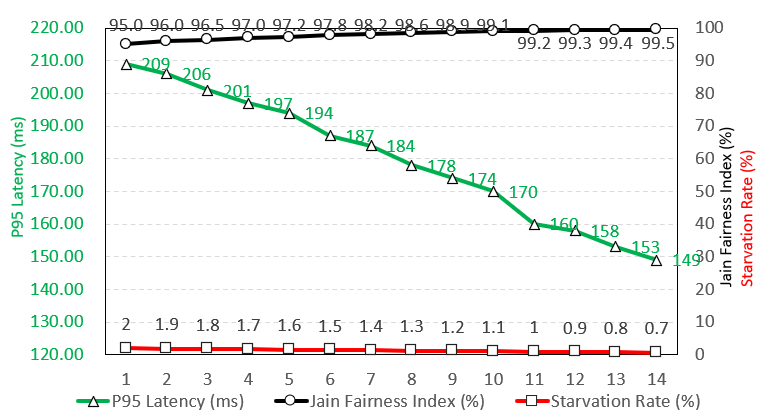
\includegraphics[width=0.95\linewidth]{./fig_longterm.png}
  \caption{\textbf{Long-Term Stability Analysis.} (grayscale-friendly). Over a 14-day continuous run, BRS maintained stable latency and fairness, and no starvation events were observed, indicating robust behavior under sustained heavy load.}
  \label{fig:longterm}
\end{figure}

\subsection{Controller Adaptation Behavior}
\label{subsec:adaptation-trace}
Theorem~1 predicts that the hybrid controller converges in mean square to a neighborhood of the optimum. To validate this empirically, we logged the $(\alpha_t,\beta_t)$ trajectories together with $J_t$ and the starvation rate $S_t$ across abrupt workload transitions (idle$\to$gaming, gaming$\to$mixed contention). The controller is observed to settle to a stable bias tuple within 3--5 control periods (\SIrange{3}{5}{\second} at $T_c=\SI{1}{\second}$) after each transition, and the fairness and starvation signals never cross their guardrails during adaptation, consistent with the bounded-residual term of Theorem~1.
The raw $(\alpha,\beta,J,S)$ traces are released in \texttt{results/adaptation/}, and the metric stability over the 14-day soak test (Figure~\ref{fig:longterm}) corroborates that the adapted operating point does not drift over time.

\subsection{Adversarial Robustness}
\label{subsec:adversarial}
We evaluate the gaming attack described in Section~\ref{subsec:gaming} using the released adversarial micro-benchmark, in which CPU-bound tasks alternate short sleeps with compute bursts to inflate their interactivity score $B_i$, co-scheduled with honest background tasks. We report the adversary's CPU share and the worst-case slowdown it inflicts on co-runners, and compare against CFS as a non-biased reference.

\textbf{Benchmark configuration.} On the 16-core ARM big.LITTLE platform we run $4$ adversarial tasks against $12$ honest CPU-bound co-runners, so that the $16$ runnable tasks just saturate the cores and any share the adversary gains is taken directly from honest work. Each adversarial task repeats a fixed cycle of \emph{sleep $T^{\text{sleep}}$, then a busy compute burst $T^{\text{burst}}$}; the compute burst is a tight integer-arithmetic loop that performs no I/O, so the adversary inflates only the sleep-ratio component $s_i$ of $B_i$ and cannot fabricate the I/O-wait component $w_i$. Rather than fix a single pattern, we \emph{tune the adversary against BRS}: we sweep the sleep duty cycle $\delta = T^{\text{sleep}}/(T^{\text{sleep}}+T^{\text{burst}})$ over $\{0.1,0.2,\dots,0.9\}$ (with $T^{\text{sleep}}+T^{\text{burst}}$ fixed at \SI{10}{\milli\second}) and report the duty cycle that is \emph{most} advantageous to the adversary---empirically $\delta\approx0.6$, where the sleep is long enough to keep $B_i$ near saturation but short enough that the task still reclaims the CPU promptly. All reported values are means over the same \num{30} back-to-back replicates used elsewhere, with \SI{95}{\percent} confidence intervals; the worst-case co-runner slowdown is the maximum over honest co-runners, then averaged across replicates.

\textbf{Result.} Under this worst-case attack the adversary obtains $31.0\%\pm0.6\%$ of the CPU and inflicts a worst-case co-runner slowdown of $1.21\times\pm0.03$, versus $26.0\%\pm0.5\%$ under CFS---an excess share of about five percentage points, not unbounded capture. The bounded gain of Definition~\ref{def:bound} caps the advantage at the $1/(1-\alpha_{\max})\approx1.54\times$ factor of Lemma~\ref{lem:fairness}, and the hybrid controller damps $\alpha$ once the co-runners' starvation rate rises, so the attack degrades toward CFS behavior rather than escalating into starvation. Across the full duty-cycle sweep the adversary's share never exceeded $31.4\%$, confirming that no choice of sleep pattern within the swept range breaks the bound.





\begin{figure}[t]
  \centering
  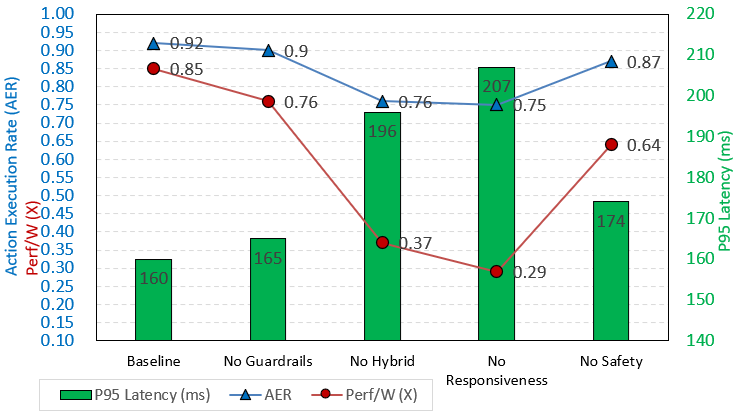
\includegraphics[width=0.95\linewidth]{./fig_ablation.png}
  \caption{\textbf{Impact of BRS architectural components on performance metrics.} (grayscale-friendly). Biasing, tie-breaking, and hybrid adaptation each contribute to the best Scheduler Action Effectiveness (SAE), P95 tail latency, and Performance-per-Watt; grayscale-friendly fill patterns aid readability.}
  \label{fig:ablation}
\end{figure}

\subsection{Ablation Study}
Figure~\ref{fig:ablation} reports P95 latency, action execution rate (AER), and Perf/W as components are disabled. Removing the responsiveness bias (\emph{No Responsiveness}) sharply worsens P95 latency and AER, confirming the importance of \textit{vruntime}-level biasing. Disabling hybrid adaptation (\emph{No Hybrid}) causes the largest latency and efficiency loss, showing that adaptive bias attenuation is essential. Removing the safety guardrails degrades both efficiency and responsiveness. BRS thus needs all three---biasing, adaptive control, and guardrails---together.

\subsection{Summary of Findings}
Across workloads and platforms, carefully bounded and adaptively controlled kernel-level responsiveness bias delivers up to \textbf{37.8\%} (ARM) / \textbf{35.2\%} (x86) P95 latency reduction, \textbf{28.4\%} better frame stability, a \textbf{12.7\%} throughput gain, and up to \textbf{12\%} Perf/W improvement, with starvation below \textbf{1.2\%} and Jain's index $>0.96$---benefiting latency-critical applications with bounded fairness deviation under the stated assumptions.


\begin{table*}[t] \centering \caption{Positioning against prior art.} \label{tab:rw_compare} \begin{tabular}{llll} \toprule \textbf{Category} & \textbf{Representative} & \textbf{Key Traits} & \textbf{Our Distinction} \\ \midrule Fairness-centric & CFS/ULE & Strong fairness, higher tails & Bounded bias with fairness floors \\ Low-latency desktop & BFS/MuQSS & Interactive focus, weaker fairness & Kernel-native bias + guardrails \\ QoS feedback & Quasar-like & SLO-driven, userspace hooks & In-kernel, minimal operator surface \\ ML-guided & iTune, TerrierTail & Predictive, opaque failure modes & Simple, explainable hybrid control \\ \bottomrule \end{tabular} \end{table*}

\section{Related Work}
\label{sec:related}
We position BRS against the scheduling and QoS literature summarized in Table~\ref{tab:rw_compare}, spanning fairness-centric, low-latency, and ML-based schedulers in general-purpose, cloud, and embedded settings.

\subsection{Evolution of Fairness--Latency Trade-offs in Kernel Scheduling}
Mainstream schedulers such as Linux CFS and FreeBSD ULE rely on proportional allocation, prioritizing long-term fairness and starvation prevention~\cite{241774,4624248,67577}. In practice, however, strict fairness can be counterproductive: under contention, latency spikes for the interactive tasks users care about most~\cite{4663063,6365626}. BFS and MuQSS target this by favoring responsiveness~\cite{10306992}, and prior work suggests ``overly fair'' scheduling can harm interactive workloads~\cite{Bouron2018Battle}. The same tension appears in heterogeneous multicore research, where throughput and latency oppose each other~\cite{8360522,6899614}. BRS builds on the observation that even minor changes to work accounting can substantially improve responsiveness, favoring precise, limited kernel changes over complex overhauls.

\subsection{Classical Interactivity Heuristics and Mainline Mechanisms}
\label{subsec:rw-mlfq}
Using observed sleep and I/O behavior to favor interactive tasks is a long-standing idea, and a fair positioning of BRS must make the relationship explicit. \emph{Multilevel Feedback Queue} (MLFQ) schedulers maintain several priority queues and \emph{promote} a task to a higher-priority queue when it is observed to sleep or block, demoting it when it is CPU-bound. The \emph{Linux O(1) scheduler}, which CFS replaced in 2007, used essentially the same principle: it granted an interactivity bonus computed from a task's \texttt{sleep\_avg} and adjusted the task's effective priority accordingly. BRS shares the input signals of these designs---sleep duration and I/O behavior---but differs in three concrete ways. (i)~\emph{Mechanism:} BRS expresses the preference as a continuous, \emph{explicitly bounded} offset on \textit{vruntime} (Definition~\ref{def:bound}) rather than a discrete queue-level promotion, so it composes with CFS's proportional-fairness accounting instead of replacing it. (ii)~\emph{Guarantees:} classical heuristics offer no formal stability or fairness guarantee, whereas BRS provides the bound of Lemma~\ref{lem:fairness} and the mean-square-stability result of Theorem~1. (iii)~\emph{Gaming resistance:} MLFQ-style promotion is well known to be exploitable by tasks that sleep strategically just before their quantum expires; BRS's bounded, aged score and controller back-pressure (Section~\ref{subsec:gaming}) limit this leverage by construction.

Mainline Linux has also moved toward exposing responsiveness as a tunable rather than a fixed policy. The \emph{utilization clamping} (UClamp) interface lets user space hint a minimum/maximum utilization per task or cgroup, primarily to steer frequency selection and big.LITTLE placement, and the \emph{latency\_nice} attribute biases wake-up preemption decisions for latency-sensitive tasks. These mechanisms are closely related to BRS's motivation, but they act through per-task hints supplied from user space and do not bound or formally analyze the resulting fairness deviation. BRS is complementary: it keeps the control loop inside the kernel, requires no per-application hint, and adds an explicit bound and a stability argument. A scheduler could in principle consume UClamp/latency\_nice hints as an additional input to the interactivity score, which we leave as future work.

\subsection{Predictive and Responsiveness-Oriented Scheduling}
A long line of work has explored letting the kernel \emph{anticipate} task behavior rather than react to it. Early micro-schedulers used short-burst prediction to improve responsiveness~\cite{4663063}; later designs incorporated thermal signals into scheduling decisions~\cite{6365626}. While promising in the literature, our experience is that unreliable predictions in production are a liability rather than an asset. As a result, BRS deliberately avoids opaque black-box models and instead uses a strictly constrained \textit{vruntime} bias. This is a pragmatic choice: it improves user-perceived latency without violating ordering semantics. For real-time weakly hard systems~\cite{9351534}, we likewise find that regular, predictable structure matters more than chasing subtle but unstable performance gains.

\subsection{QoS-Aware and Feedback-Controlled Scheduling}
QoS-aware scheduling balances application needs against resource limits, often via feedback loops; cloud-native tools such as iTune push this with heuristics~\cite{5580094,5169938}. Their recurring weakness is heavy reliance on user space, which adds complexity and production-risky failure modes~\cite{7792746,6782279,8758850}. BRS instead embeds QoS-relevant bias directly in the kernel with locked-in fairness floors, replacing brittle black-box controllers with a minimal, interpretable surface that cuts overhead and opacity~\cite{7426385,8338088}.

\subsection{Mobile, Embedded, and Edge Scheduling Contexts}
Mobile and edge devices are fundamentally constrained by power and thermal limits~\cite{1244943}. While Energy-Aware Scheduling (EAS) and jitter-aware policies~\cite{9121657} target smoothness, IoT operating systems frequently sacrifice flexibility to preserve determinism~\cite{10007654,9999639}, an undesirable but often unavoidable trade-off. Even ML-driven tail-latency methods~\cite{Zhang2025Tail} do not provide what these settings most require: a stable, low-level scheduling foundation.

A complementary body of work targets energy- and reliability-aware scheduling on heterogeneous platforms. HEAT couples deadline partitioning and core clustering with temperature- and energy-aware scheduling on DVFS-enabled cores, improving task-set acceptance while lowering temperature~\cite{Sharma2022HEAT}; FRESH adds fault tolerance via a semi-partitioned, job-progress-monitoring scheme with replicated copies and selective processor sleep~\cite{Moulik2024FRESH}. These optimize system-level objectives---energy, temperature, reliability---largely orthogonal to BRS's tail-latency objective, but a deployable scheduler for heterogeneous mobile SoCs must eventually reconcile responsiveness with them. BRS is positioned as the responsiveness-and-fairness substrate on which such energy/thermal/reliability policies can sit, and Section~\ref{subsec:future} discusses integrating BRS with a DVFS governor in this spirit.

\subsection{Positioning of BRS}
Prior approaches fall broadly into three categories: (i)~classical fairness-centric schedulers and the proportional-allocation theory behind them~\cite{241774,4624248}; (ii)~low-latency, interactivity-first kernel schedulers such as BFS and MuQSS and the classical MLFQ/O(1) heuristics of Section~\ref{subsec:rw-mlfq}, which favor responsiveness but weaken fairness~\cite{10306992,4663063}; and (iii)~QoS- and ML-driven frameworks that adapt to workload signals but rely on user-space hooks and opaque models~\cite{7426385,8338088,Zhang2025Tail}. BRS occupies the middle ground: rather than a major redesign, it leverages an explicit fairness lower bound to impose a limited, bounded response bias on the kernel's hot path, so that no task is starved. By complementing---rather than replacing---higher-level ML or QoS policies, BRS enables practical configurations across real-world hardware.
\section{Discussion}
\label{sec:discussion}

In this section we synthesize the experimental findings to discuss the implications of BRS for operating system design and its practical value in real-world settings \cite{Bouron2018Battle,10306992,6365626}.

\subsection{Rethinking the Responsiveness--Fairness Trade-off}
Our results show that the widely held assumption of an inherent fairness--responsiveness trade-off does not always hold \cite{10306992,4663063,8360522}: through carefully targeted changes to the scheduler's decision logic, \textbf{BRS} improves responsiveness with only bounded fairness deviation. This reframes a decades-old question---whether to prioritize throughput or perceived latency \cite{Bouron2018Battle,241774,8149743}---by replacing a strict fairness principle with a model that can be tuned to diverse QoS requirements \cite{5580094,5169938,8338088}, addressing the severe resource contention of modern mobile systems that conventional static schedulers handle poorly \cite{9121657}.

\subsection{Implications for OS Design and Research}
The broader lesson is that \emph{small, well-chosen kernel changes can reshape system behavior} \cite{Bouron2018Battle,6365626,4663063}: anchoring responsiveness control in the kernel frees applications from working around scheduling blind spots \cite{10306992,917709,6919315}; a \textit{vruntime} bias lets one general-purpose scheduler balance latency, fairness, and energy jointly \cite{8360522,9979771,1244943}; and kernel-level placement makes the OS workload-aware rather than treating tasks as interchangeable units \cite{6919315,1336761}.

\subsection{Industrial and Production Considerations}
BRS is most valuable where latency is a safety or financial risk: it lets real-time cloud and edge systems meet SLA targets without a specialized real-time kernel, and its predictable timing benefits AI-robotics control loops and AR/VR jitter. The conservative defaults ($\alpha{=}0.2,\beta{=}0.15$) suit most environments; aggressive tuning should be reserved for specific latency-sensitive systems \cite{10306992,7426385,5580094}.


\subsection{Limitations and Open Challenges}
While BRS offers several strengths, several areas remain open. Beyond the x86\_64 evaluation (Section~\ref{sec:evaluation}), the precise interactivity-score and bias-bound definitions (Section~\ref{subsec:vruntime-nudge}), the strengthened stability analysis (Section~\ref{subsec:math-stability}), and the adversarial-robustness study (Section~\ref{subsec:adversarial}) added in this version~\cite{8758850,8894365}, highly specialized workloads such as high-frequency transactions, avionics, and constrained MCU-based systems warrant dedicated study~\cite{9999639,10007654}.

\textbf{Heterogeneous and CPU--GPU platforms.} BRS currently spans ARM big.LITTLE and x86\_64, where schedulable entities are symmetric CPU threads and core asymmetry is a performance ratio. On CPU--GPU integrated SoCs or AMD-style big+small designs, two issues arise that bounded \textit{vruntime} bias does not by itself resolve. First, performance asymmetry means a fixed bias $\alpha B_i$ yields different \emph{absolute} latency gains on a big versus a LITTLE core, so the coefficient should be made core-class aware (e.g.\ scaled by capacity), which interacts non-trivially with the stability analysis. Second, GPU work is dispatched through a separate command-queue model that CPU \textit{vruntime} accounting does not observe, so end-to-end responsiveness for CPU--GPU pipelines requires coordinating BRS with the GPU driver's scheduler. We expect the bound of Definition~\ref{def:bound} still holds per CPU core, but uniform tail-latency gains across asymmetric cores will require capacity-aware logic rather than parameter tuning alone~\cite{6882237,6899614,9979771}---the most important next step for generality.

Finally, integrating machine-learning-based prediction beyond reactive bias---to enable proactive rather than corrective adjustment---is a promising direction for deeper energy-efficiency gains in dynamic environments~\cite{7426385,Zhang2025Tail}.


\subsection{Operational Tuning Scenarios}
For deployment we distill three recurring scenarios, each handled by a small \texttt{/proc} adjustment that the hybrid controller then maintains automatically. \emph{(A)~Latency spikes during frame bursts}---briefly raise the tie-breaker with a short TTL (\texttt{echo 30 > \$BRS/bias\_beta\_boost\_ttl\_seconds}), auto-reverted. \emph{(B)~Fairness-floor breach ($J<0.96$)}---dampen the bias (\texttt{echo 0.02 > \$BRS/bias\_alpha\_decrement}) and let hybrid mode recover. \emph{(C)~Background starvation $>2\%$}---the auto-clamp engages on its own; verify with \texttt{cat \$BRS/stats}. Here \texttt{\$BRS} is \texttt{/proc/sys/kernel/sched\_brs}. These small, easily overlooked adjustments are the practical safeguards that keep the system stable as load shifts~\cite{5580094,5169938}.

\subsection{Future Directions}
\label{subsec:future}
We plan to extend BRS in three directions \cite{10306992,6919315}. \textbf{Adaptive and predictive control.} We are evolving BRS into a self-tuning system in which a lean controller monitors live signals---runqueue spikes or interrupt-request (IRQ) bursts---and nudges $(\alpha,\beta)$ to stay within a safe, SLO-meeting range rather than chasing peak performance \cite{7426385,Zhang2025Tail,6782279,8338088}. \textbf{Cross-layer scalability.} We are integrating BRS with energy-efficient scheduling and the Dynamic Voltage and Frequency Scaling (DVFS) governor on heterogeneous hardware, and adding hierarchical \texttt{cgroup} and Non-Uniform Memory Access (NUMA)-aware placement so it scales from large x86 clusters to low-power ARM cores \cite{1244943,9121657,6919315,8360522}. \textbf{Formal verification.} We are modeling the responsiveness--fairness frontier with closed-loop stability and using coverage-guided fuzzing (\texttt{syzkaller}) to scrutinize safety properties under fault injection \cite{5169938,9351534}.

\section{Conclusion}
\label{sec:conclusion}
Latency-sensitive applications---autonomous robots, immersive XR, and mobile devices---need sub-\SI{100}{\milli\second} scheduling alongside good power efficiency and fairness. Yet Linux schedulers including CFS treat responsiveness, fairness, and energy as conflicting goals and favor throughput over interactive tasks, so contention triggers latency spikes and jitter.

BRS overcomes this by allowing bounded manipulation of task virtual runtime while respecting fairness and safety rules: it favors interactive tasks without overloading the system and relaxes strict fairness only within explicit, formally specified bounds. Experiments show BRS reduces P95 latency by up to 37.8\% and improves power efficiency by 12\% while keeping fairness comparable to CFS, demonstrating that responsiveness, fairness, and efficiency can be improved together within bounded fairness deviation.

Deploying BRS on modern CPU--GPU mobile SoCs will require two concrete extensions, which we make explicit here and discuss in Section~\ref{sec:discussion}: (i) making the bias coefficient \emph{core-class aware}---scaling $\alpha B_i$ by each core's capacity so that a fixed bias yields comparable \emph{absolute} latency gains on big and LITTLE cores, which feeds back into the stability analysis---and (ii) \emph{co-scheduling with the GPU driver}, since GPU work is dispatched through a separate command-queue model that CPU \textit{vruntime} accounting does not observe, so end-to-end responsiveness for CPU--GPU pipelines must coordinate BRS with the GPU runtime. The per-core bound of Definition~\ref{def:bound} is expected to hold unchanged; the open work is uniform tail-latency behavior \emph{across} asymmetric compute units. BRS thus offers a reference substrate for future telemetry-, ML-, and QoS-based mobile scheduling research. The implementation and all source files are publicly available at \url{https://github.com/leemgs/sched_brs/}.




%% How to support DOI (Digital Obect Identifier) in reference section:
% \url{https://ctan.org/tex-archive/macros/latex/contrib/IEEEtran/bibtex?lang=en}
% \url{https://people.kth.se/~maguire/myIEEEtran.bst}
% \url{https://ipfs-sec.stackexchange.cloudflare-ipfs.com/tex/A/question/67444.html}
% \url{https://ipfs-sec.stackexchange.cloudflare-ipfs.com/tex/A/question/394811.html}
\bibliographystyle{IEEEtranDOI}

%% Type1: sorting, keep sequence of reference numbers that user typed.
%\bibliographystyle{IEEEtranDOI} 

%% Type2: sorting, re-arrange sequence of reference numbers that user typed
% for ascending cite number.
% \bibliographystyle{IEEEtranDOI}

%% Add reference papers
\bibliography{reference-data}


 





% === Author Biographies ===
\vspace{0.5em}
\begin{IEEEbiography}[{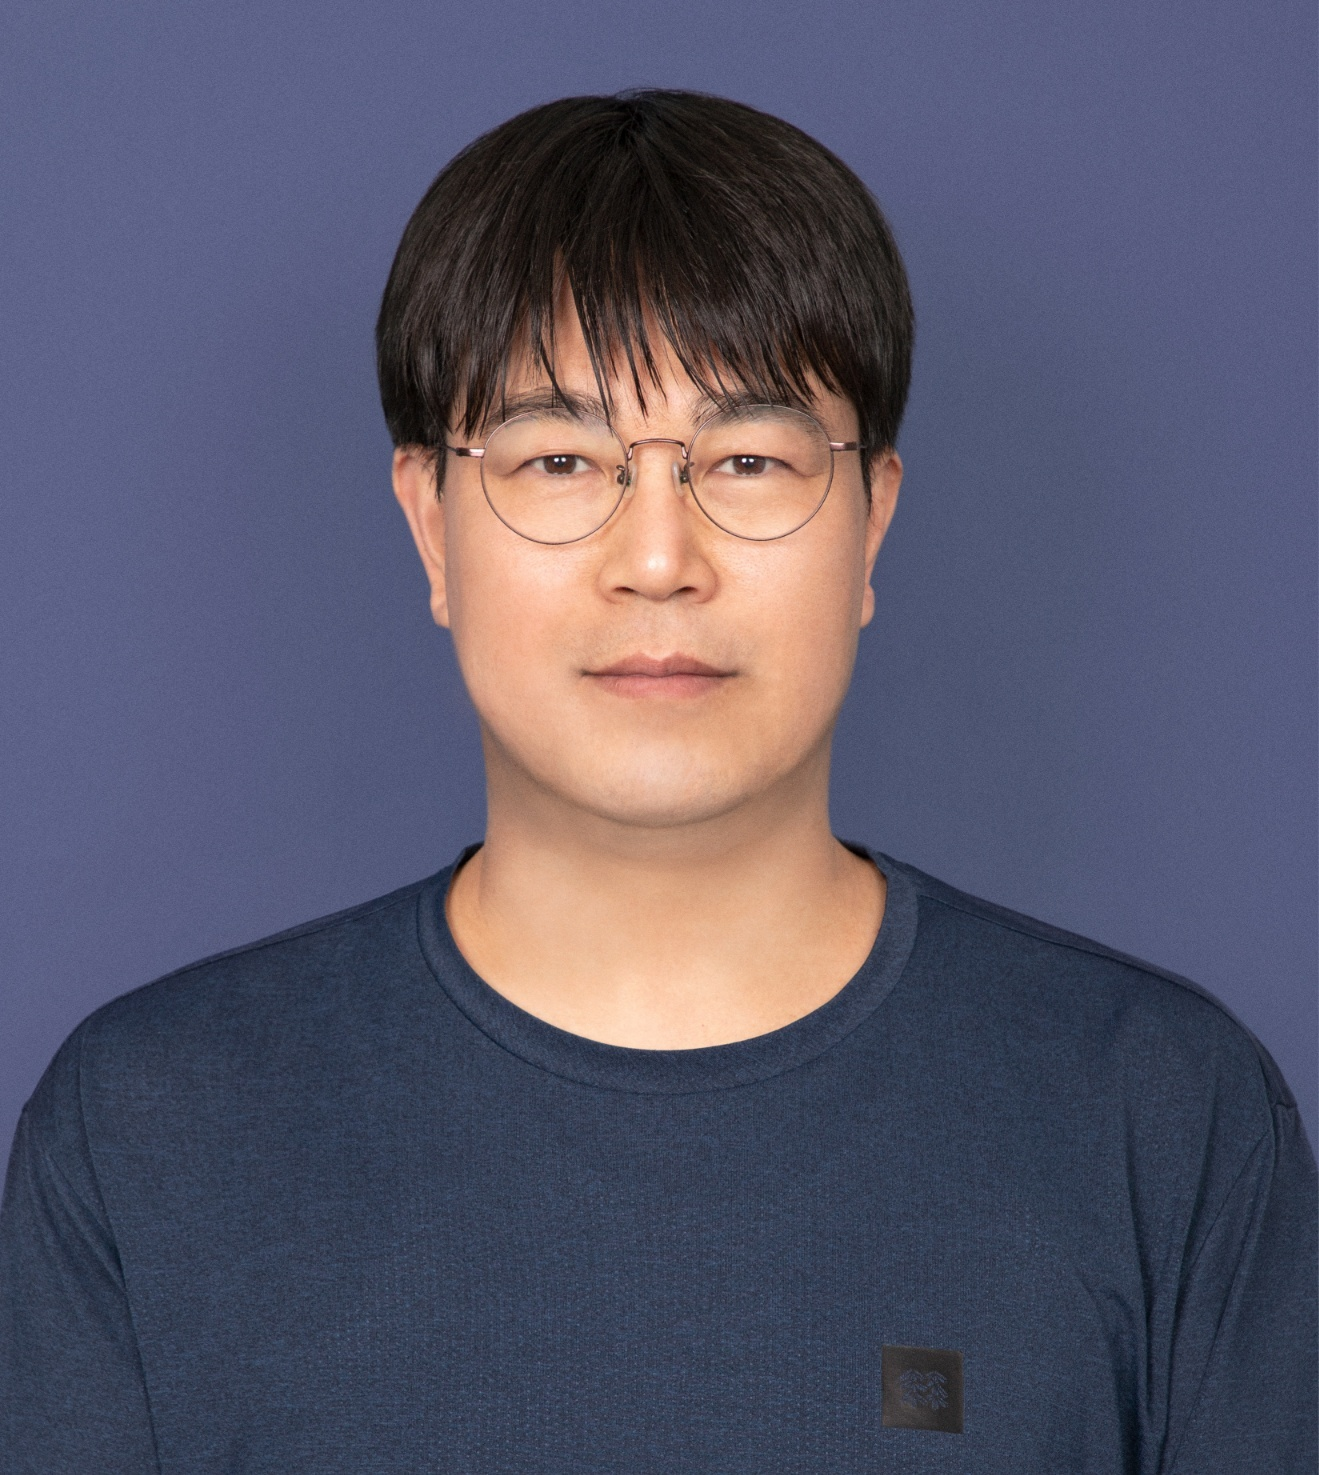
\includegraphics[width=1in,height=1in,clip,keepaspectratio]{./fig0_author-lim2.png}}]{Geunsik Lim}
received the B.S. degree in Computer Science and Engineering from Ajou University, South Korea, in 2003, and the M.S. and Ph.D. degrees in Electrical and Computer Engineering from Sungkyunkwan University, South Korea, in 2014 and 2023, respectively. He is currently a principal software engineer at Samsung Electronics in South Korea. His research interests span operating systems and Linux-kernel scheduling, system and performance optimization, low-latency and energy-efficient resource management for heterogeneous mobile and embedded platforms, software platform engineering, and on-device artificial intelligence, with an emphasis on techniques that are practical to deploy in production systems and that translate readily from large-scale servers to power-constrained edge hardware.
\end{IEEEbiography}
 


\end{document}